%%%%%%%%%%%%%%%%%%%%%%%%%%%%%%%%%%%%%%%%%
% University Assignment Title Page 
% LaTeX Template
% Version 1.0 (27/12/12)
%
% This template has been downloaded from:
% http://www.LaTeXTemplates.com
%
% Original author:
% WikiBooks (http://en.wikibooks.org/wiki/LaTeX/Title_Creation)
%
% License:
% CC BY-NC-SA 3.0 (http://creativecommons.org/licenses/by-nc-sa/3.0/)
% 
% Instructions for using this template:
% This title page is capable of being compiled as is. This is not useful for 
% including it in another document. To do this, you have two options: 
%
% 1) Copy/paste everything between \begin{document} and \end{document} 
% starting at \begin{titlepage} and paste this into another LaTeX file where you 
% want your title page.
% OR
% 2) Remove everything outside the \begin{titlepage} and \end{titlepage} and 
% move this file to the same directory as the LaTeX file you wish to add it to. 
% Then add \input{./title_page_1.tex} to your LaTeX file where you want your
% title page.
%
%%%%%%%%%%%%%%%%%%%%%%%%%%%%%%%%%%%%%%%%%
%\title{Title page with logo}
%----------------------------------------------------------------------------------------
%	PACKAGES AND OTHER DOCUMENT CONFIGURATIONS
%----------------------------------------------------------------------------------------
\documentclass[12pt]{article}
\usepackage[spanish, es-tabla]{babel}
\usepackage[utf8x]{inputenc}
\usepackage{amsmath}
\usepackage{graphicx}
\usepackage[colorinlistoftodos]{todonotes}
\usepackage{makeidx}
\usepackage[colorlinks=true,linkcolor=black,anchorcolor=black,citecolor=black,filecolor=black,menucolor=black,runcolor=black,urlcolor=blue]{hyperref}
\usepackage{color}
\usepackage{caption}
\usepackage{etoolbox}
\usepackage{fancybox}
\usepackage{enumitem}
\usepackage{listings}
\lstset{
	language=sh,
	breaklines=true,
	breakatwhitespace=true,
	basicstyle=\ttfamily,
	showstringspaces=false,
	columns=fullflexible-
}
\usepackage{booktabs}
\usepackage{tabularx}
\usepackage{lipsum}

\newcommand\pro{\item[$+$]}
\newcommand\con{\item[$-$]}

\newcommand{\icon}[1]{\includegraphics[height=18pt]{#1}}
\robustify{\icon}
\makeindex
\graphicspath{{./img/}}

\begin{document}

\renewcommand\indexname{Índice}
\begin{titlepage}

\newcommand{\HRule}{\rule{\linewidth}{0.5mm}} % Defines a new command for the horizontal lines, change thickness here

\center % Center everything on the page
 
%----------------------------------------------------------------------------------------
%	HEADING SECTIONS
%----------------------------------------------------------------------------------------

\textsc{\LARGE Facultad de Informática}\\[1.5cm] % Name of your university/college
\textsc{\large Adrián García García}\\[0.5cm] % Minor heading such as course title

%----------------------------------------------------------------------------------------
%	TITLE SECTION
%----------------------------------------------------------------------------------------

\HRule \\[0.4cm]
{ \huge \bfseries Arquitecturas Cloud y microservicios}\\[0.4cm] % Title of your document
\HRule \\[1.5cm]
 
%----------------------------------------------------------------------------------------
%	AUTHOR SECTION
%----------------------------------------------------------------------------------------


% If you don't want a supervisor, uncomment the two lines below and remove the section above
%\Large \emph{Author:}\\
%John \textsc{Smith}\\[3cm] % Your name

%----------------------------------------------------------------------------------------
%	DATE SECTION
%----------------------------------------------------------------------------------------

{\large \today}\\[2cm] % Date, change the \today to a set date if you want to be precise

%----------------------------------------------------------------------------------------
%	LOGO SECTION
%----------------------------------------------------------------------------------------


\includegraphics[width=4cm,keepaspectratio]{logo.png}
 
%----------------------------------------------------------------------------------------

\vfill % Fill the rest of the page with whitespace



\captionsetup[figure]{labelformat=empty,justification=raggedright,singlelinecheck=false}
% Include image from images directory
\begin{figure}[h]

        
\includegraphics[width=2cm,keepaspectratio]{cc-by-sa.png}
        \label{fig:by-sa}
        \caption{ This work is licensed under a \href{https://creativecommons.org/licenses/by/4.0/legalcode}{CC-BY-SA 4.0 License}.}

\end{figure}

\end{titlepage}

\tableofcontents
\clearpage

\begin{abstract}
Este trabajo tiene como objetivo exponer y profundizar en los conceptos expuestos en una conferencia optativa que tuvo lugar durante la semana de la informática de 2017. Los ponentes fueron dos ingenieros de la empresa GMV (Ricardo de Castro y Roberto Galán). En concreto, el nombre de la conferencia era el siguiente: Despliegue automático de arquitecturas escalables basadas en microservicios sobre el Cloud de Google (23 de Febrero, 11-14 horas). Conviene puntualizar que al final no usaron la plataforma de Google, sino que se basaron en Amazon Web Services y Docker Swarm para desplegar una aplicación web que hacía uso de microservicios para su funcionamiento. Al mismo tiempo, hablaron de un concepto que está muy de moda últimamente como es el enfoque \emph{DevOps}, también está relacionado con el despliegue rápido y eficiente de código en la nube, la automatización de procesos de desarrollo (\textit{testing}, recogida de métricas, despliegue, etc.) y las metodologías ágiles.
\end{abstract}

\section{Introducción}\label{sec:intro}


En primer lugar, expondré diferentes conceptos que considero relevantes tanto en el campo del \emph{Cloud Computing} como en el diseño de aplicaciones empresariales que se ejecutan en servicios web, que en general presentan un alto grado de complejidad y número de componentes. 

Durante la conferencia, se hizo especial hincapié en las necesidades de los clientes y las características que estos exigen en una aplicación de carácter empresarial que se ejecuta en la nube, aunque se mencionaron brevemente, más tarde encontré diferentes enlaces con más información sobre el tema en~\cite{reliab}. Los requisitos más destacados son los siguientes:

\begin{itemize}
\item \textbf{Fiabilidad}. El funcionamiento de las aplicaciones web está íntimamente relacionado con la imagen que las grandes empresas tienen en la sociedad, si una tienda de comercio electrónico se cae durante una hora puede suponer pérdidas millonarias para la empresa y acarrea el riesgo de que sus clientes dejen de confiar en ella y se pasen a la competencia. Debido a esto, los clientes esperan que su aplicación tenga el mínimo número de errores posibles. Uno de los aspectos más importantes en este sentido es que se haga un proceso meticuloso de \textit{testing} y validación antes de publicar una aplicación, priorizando las partes más críticas del sistema y que pueden suponer un cuello de botella para la misma.
\item \textbf{Recuperación instantánea ante fallos} (\emph{Zero Down Time}~\cite{zdwt}). En caso de que la aplicación llegue a fallar, lo que es imposible de evitar al completo, es necesario minimizar el tiempo en el que no se provee un servicio. Asegurar un tiempo mínimo de recuperación supone un desafío importante cuando una máquina física actúa como el punto de fallo único de la aplicación (\textit{Single Point of Failure}). Sin embargo, el hecho de tener una aplicación desplegada en contenedores virtuales, nos facilita en gran medida asegurar un sistema tolerante a fallos. Este sistema debe constar de ciertas características, entre las que se destacan:
\begin{itemize}
\item Disponer de un \textbf{cluster de máquinas} configurado.
\item Aplicar técnicas de \textbf{replicación y balanceo de carga}.
\item Tener montado un \textbf{volumen compartido de datos} que permita a diferentes máquinas acceder a las imágenes que utilizan las máquinas virtuales. Por ejemplo, \emph{Network File System} (\textbf{NFS}).
\end{itemize}
\begin{figure}
\centering
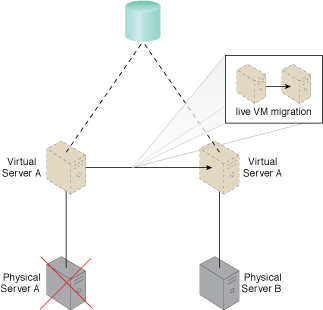
\includegraphics[width=0.5\textwidth]{spof.png}
\caption{\label{fig:zerodt}Esquema de recuperación ante fallos.}
\end{figure}
Cómo se puede observar en la Figura~\ref{fig:zerodt}, cuando el servidor físico A falla, se desencadena una migración del contenedor virtual al servidor B. Lo que debería ocurrir sin complicaciones en caso de que el volumen de datos compartido por red siga disponible y solo haya ocurrido un problema aislado en la máquina A. En general, el demonio encargado de vigilar el correcto funcionamiento de los nodos se denomina \textit{watchdog} y su funcionamiento se basa en el intercambio periódico de mensajes con los nodos del cluster para intercambiar información del estado del servicio (\textit{keepalive o hearbeat}).
\item \textbf{Tiempo rápido de despliegue}. Uno de los problemas más extendidos en el ámbito de las aplicaciones empresariales de elevada complejidad es que la aplicación puede tener muchas dependencias entre diferentes componentes, lo que hace difícil realizar un despliegue limpio y sin errores. Se ponía como ejemplo el clásico problema de que en el entorno de desarrollo funciona todo perfectamente, pero cuando se traslada a producción deja de hacerlo y cada equipo le echa la culpa a otro.
\item \textbf{Escalabilidad}. Los servicios pueden recibir grandes picos de tráfico y deben ser capaces de responder ante los mismos sin errores. Es evidente que la optimización de cada componente de la aplicación es un aspecto importante, pero además se debe diseñar un sistema capaz de balancear la carga y aumentar la dedicación de recursos replicando sus unidades de cómputo para responder ante los incrementos en demanda. Esto es relativamente fácil de hacer en entornos cloud o con soluciones de virtualización como Docker.
\end{itemize}

Este trabajo está estructurado de la siguiente forma, en la Sección~\ref{sec:cloud} se realizará una exposición de diferentes conceptos que se utilizan en \emph{Cloud Computing}. A continuación se introducirá el paradigma de las arquitecturas orientadas a servicios (SOA) en la Sección~\ref{sec:soa}. Más adelante se introducirá la herramienta de contenedores Docker (Sección~\ref{sec:docker}), con la que se pueden construir de forma sencilla diferentes tipos de aplicaciones basadas en microservicios. Tras esto, en la Sección~\ref{sec:devops} Para finalizar, en la Sección~\ref{sec:conclu} presentaré una serie de opiniones personales que se han originado a partir de la conferencia y de la investigación posterior realizada.

\section{Cloud Computing}\label{sec:cloud}
A continuación se presentarán diferentes conceptos utilizados en el diseño y construcción de aplicaciones que se ejecutan servicios alojados la nube, concepto que se refiere a el alquiler de servidores o servicios específicos a un proveedor externo en función de nuestras necesidades de cómputo, este paradigma es comúnmente conocido como \emph{Cloud Computing}. El Instituto Nacional de Estándares y Tecnología de Estados Unidos (NIST) publicó en 2002 una serie de principios de diseño y definiciones de \emph{Cloud Computing}~\cite{cloudfunds}. Algunos de las propiedades esenciales que pueden variar de un proveedor de servicio a otro son las siguientes:

\begin{itemize}
\item \textbf{Servicio bajo demanda auto-escalable}. Un cliente obtiene unas capacidades de cómputo como tiempo de un servidor o almacenamiento en red en función de sus necesidades sin requerir interacción humana con el proveedor de servicio.
\item \textbf{Disponibilidad de recursos}. Los recursos ofrecidos por el proveedor son ofrecidos a múltiples clientes, que comparten infraestructura pero cada uno dispone de una diferente asignación de recursos físicos y virtuales. Hay cierta sensación de incertidumbre en cuanto a la localización del servicio. Sin embargo, muchos proveedores permiten especificar a alto nivel la región, país o incluso \textit{datacenter} en el que se ejecutará la aplicación. En general, los clientes pueden escoger ente diferentes planes de pago, que permiten adaptar a nuestras necesidades la capacidad de almacenamiento, el tipo (HDD vs SSD), la memoria RAM, el procesador, el ancho de banda o incluso la arquitectura en la que se ejecutará nuestra aplicación (cada vez más proveedores permiten que nuestra aplicación haga uso de GPUs y otros aceleradores).
\item \textbf{Servicio de conexión multiplataforma con un alto ancho de banda}. Pongamos el ejemplo de una pequeña o mediana empresa (incluso una grande para un proyecto con necesidades variables a lo largo del tiempo), el coste de adquirir y mantener un conjunto de servidores propios para desplegar una aplicación en muchas ocasiones no deriva un beneficio suficiente para rentabilizar la inversión. Sin embargo, las capacidades del servicio ofrecidas a través de la red por los proveedores Cloud se adaptan a tus necesidades, tienen una calidad de servicio similar a la de un ISP (\textit{Internet Service Providers}) y disponen de una infraestructura con un diseño de alta eficiencia energética. Además, se ocupan de toda la infraestructura y seguridad para que las aplicaciones sean accedidas mediante mecanismos estándar (HTTP) y en plataformas heterogéneas (móviles, tablets, portátiles, servidores, etc.).
\item \textbf{Recolección de métricas}. Los sistemas Cloud controlan y optimizan automáticamente el uso de recursos a través de la recolección de diferentes métricas de rendimiento (ancho de banda, porcentaje de USO de CPU y disco, cuentas de usuario activas, etc.). Además, se suelen aportar diferentes herramientas de visualización como los \textit{dashboards}, que permiten a los usuarios tomar decisiones sobre el tipo de servicio que se ajusta más a sus necesidades.
\end{itemize}

En función del modelo de servicio que nos ofrezca cada proveedor, podemos clasificar los servicios Cloud en 3 clases fundamentales:

\begin{itemize}
\item \textbf{Software as a Service} (SaaS). Este modelo representa a los servicios prestados por diferentes aplicaciones que se ejecutan en una infraestructura Cloud. Las aplicaciones pueden ser accedidas simultáneamente por múltiples clientes a través de un programa o un navegador (Ej. GitHub o Google Drive). Sin embargo, el consumidor no gestiona ni tiene el control de la infraestructura Cloud subyacente.
\item \textbf{Platform as a Service} (PaaS). Los servicios prestados al cliente se basan en el uso de lenguajes, librerías, servicios y herramientas para crear y desplegar una aplicación en una infraestructura Cloud gestionada por el proveedor. En ocasiones el cliente puede ajustar la capacidad de cómputo y controlar ciertos parámetros pero no tiene permisos de \textit{root} sobre la infraestructura. Algunos ejemplos son Microsoft Azure\footnote{Microsoft, al igual que Amazon o Google, ofrece un conjunto muy amplio de servicios que pueden ser clasificados en varias categorías. Sin embargo, se destaca la integración que Azure ofrece con las aplicaciones escritas en .NET lo que lleva a que el centro de sus servicios Cloud sean las aplicaciones en C\#.} o Google App Engine. La opción más destacada de código abierto en este ámbito se trata de Red Hat OpenShift.
\item \textbf{Infrastructure as a Service} (IaaS). Este tipo de servicio se centra en ofrecer a los clientes capacidad de procesamiento, almacenamiento, ancho de banda y otros recursos computacionales que pueden gestionarse a nivel del Sistema Operativo con control de \emph{root} y que habitualmente se encuentran en un entorno virtualizado aislado del resto de clientes a los que se provee de servicio. Algunos ejemplos son Amazon EC2 o Google Compute Engine.
\end{itemize}

Por otra parte, se pueden diferenciar varios modelos de despliegue en función de las condiciones de propiedad bajo las que se ofrece el servicio. Si la infraestructura se provee para un uso exclusivo de una única organización se trata de \emph{Private Cloud}, que puede ser propiedad de la organización o incluso ser gestionada por una diferente. También existe la posibilidad de que una comunidad de clientes que comparten ciertos objetivos (misión, requisitos de seguridad, políticas de cumplimiento de estándares, etc.) hagan uso de una misma infraestructura (\emph{Community Cloud}). Además, existen múltiples casos de infraestructuras públicas que se comparten por organizaciones académicas, gobiernos o conjuntos de empresas (\emph{Public Cloud}). Como se puede observar hay una gran variedad de modelos de propiedad y tipos de servicios; y, aunque existen múltiples alternativas, existen combinaciones de las diferentes clases que se conocen como \emph{Hybrid Cloud}.

Para más información sobre este tema y una visión completa de los patrones de diseño que se utilizan en Cloud Computing, se puede consultar este recurso~\cite{cloudpatts}.

\section{Arquitectura orientada a servicios}\label{sec:soa}
El paradigma de creación de arquitecturas orientadas a servicios, comúnmente conocido como SOA (\textbf{Service Oriented Architecture}), trata de definir aplicaciones basadas en el uso de una \textbf{colección servicios que pueden trabajar de forma autónoma}, pero que también intercambian mensajes y se coordinan para cumplir una funcionalidad más compleja. Se parte del concepto de servicio, que es una funcionalidad bien definida, autocontenida y que no depende del contexto o estado de otros servicios. Por ejemplo, validar un cliente en la aplicación o proveer datos sobre el funcionamiento de la misma por causa de una petición específica (Ej. Obtener datos del producto con ID 152). La división en servicios tiene las ventajas de que la realización de \textit{tests} y la corrección de errores se puede realizar de una forma mucho más precisa, y no es necesario cambiar la aplicación completa para corregir fallos o introducir nuevas funcionalidades. Se puede obtener más información sobre los servicios web y su funcionamiento en la siguiente referencia~\cite{wscom}.

Para implementar una arquitectura orientada a servicios de forma eficiente, es necesario tener en cuenta una serie de conceptos y estrategias de diseño~\cite{ibmsoa}:
\begin{itemize}
\item Tener claro un \textbf{conjunto de servicios} con unos objetivos bien definidos que se quieran proveer a nuestros clientes o incluso de forma interna a la organización.
\item Añadir una serie de procesos de \textbf{orquestación}, \textbf{balanceo de cargas} y de \textbf{recolección de métricas} para asegurar el buen funcionamiento de los mismos.
\item Aplicar un conjunto de patrones de diseño que permita realizar un \textbf{diseño modular}, que tenga una buena \textbf{encapsulación} de los componentes, que asegure el \textbf{aislamiento}, la \textbf{reusabilidad} y la \textbf{escalabilidad}.
\item Utilizar un modelo de programación compatible con diferentes lenguajes de programación y que sea soportado por múltiples tecnologías y estándares de comunicación, por ejemplo, los \textbf{servicios REST}.
\end{itemize}

\begin{figure}
\centering
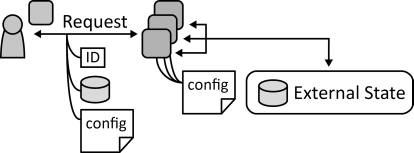
\includegraphics[width=0.5\textwidth]{stateless.png}
\caption{\label{fig:scomm}Peticiones del cliente con estado almacenado fuera de los componentes. Más información sobre componentes sin estado en~\cite{sless}.}
\end{figure}

\subsection{Comunicación}\label{sec:intro}
En una arquitectura orientada a servicios uno de los aspectos más importantes es la comunicación, ya sea entre los propios componentes de nuestra aplicación o los métodos de nuestra API que exponemos al público. Los servicios de una aplicación distribuida pueden estar alojados en diferentes máquinas, lo que hace necesario que el estado de nuestra aplicación sea almacenado de forma externa a los componentes, estos se conocen como \textbf{Stateless Components}  (puede verse un esquema en la Figura~\ref{fig:scomm}). Una de las técnicas más habituales para implementarlos es \textbf{incluir la información de estado en las peticiones} que recibe cada componente, otra forma de hacerlo sería transmitirla en los mensajes \emph{keepalive} enviados por los procesos de orquestación.

En este contexto que requiere una comunicación entre múltiples componentes sin ninguna comunicación previa de esquemas de datos, como sí era necesario con protocolos SOAP o XML, podemos destacar la utilidad de las APIs REST por las siguientes características:

\begin{itemize}
\item Representan un \textbf{protocolo cliente/servidor sin estado}.
\item \textbf{ Facilitan la portabilidad} y la comunicación entre diferentes plataformas y lenguajes, ya que se basan en el \textbf{protocolo HTTP} y el uso de sus verbos: POST, GET, PUT y DELETE.
\item Permiten \textbf{exponer recursos de forma sencilla} diferentes  mediante las URI (\textit{Unique Resource Identifier}).
\item Ofrecen una gran \textbf{flexibilidad para transmitir diferentes tipos de datos}: html, json, text, xml, jpeg, etc.
\end{itemize}

Se puede encontrar una descripción detallada de las APIs REST y sus ventajas en el blog de desarrolladores de BBVA~\cite{restapi}.

\section{Microservicios}\label{sec:micro}
%\subsection{Subsections}\index{Section}
\begin{figure}
\centering
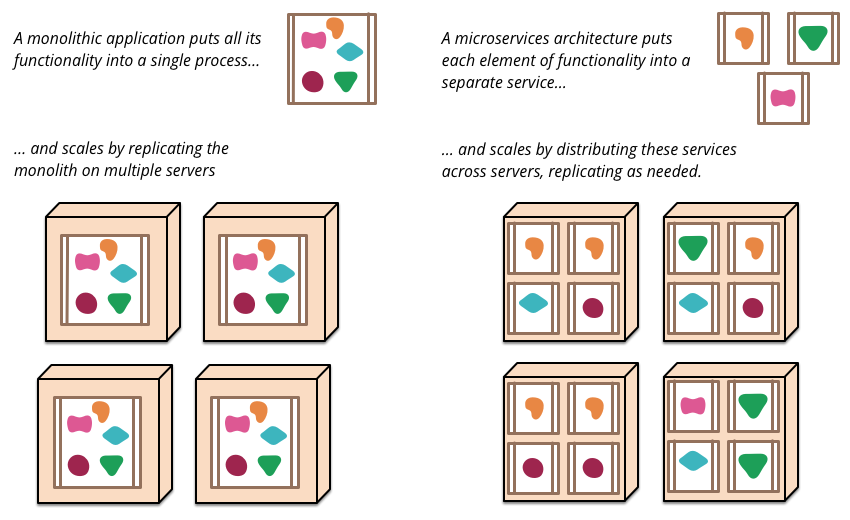
\includegraphics[width=0.9\textwidth]{sketch.png}
\caption{\label{fig:msv}Aplicación monolítica VS microservicios.}
\end{figure}

Las aplicaciones convencionales que se han desarrollado tradicionalmente para problemas tecnológico de cierta envergadura se despliegan como un solo bloque monolítico de \textit{frontend}, lógica de negocio y acceso a datos. Sin embargo, este diseño de arquitectura conlleva ciertas desventajas en el caso de necesitar escalar la capacidad de nuestra aplicación. En concreto, si existe un cuello de botella en sólo un elemento del sistema, necesitaríamos desplegar varias instancias completas de la aplicación y aplicar algún tipo de balanceo de carga para poder mejorar la latencia de respuesta. Esta es una solución pésima, ya que desperdicia recursos y no resulta eficiente para incrementar el rendimiento.

Las arquitecturas basadas en microservicios se pueden definir como un estilo de desarrollo de aplicaciones que están formadas por conjuntos de servicios pequeños y con objetivos bien definidos, que se ejecutan en máquinas diferentes y emplean mecanismos de comunicación estándar y de baja latencia. Los microservicios habitualmente se exponen como un recurso a través de una API con verbos HTTP: GET, POST, etc. En general, cada microservicio responde a peticiones sobre un elemento en particular de la lógica de negocio y existen procesos de orquestación encargados de mantener el correcto funcionamiento del sistema y escalar el número de servicios disponibles en función de la demanda.

El concepto de diseño basado en microservicios ha ganado una gran atención en los últimos años, se originó alrededor de 2014 y atrajo mucha atención hacia esta nueva forma de concebir la estructura de las aplicaciones. Puede aportar muchos beneficios si se hace uso del mismo para solucionar los problemas correctos y se comprende cuáles son sus ventajas y en qué casos sería mejor no usarlos. Uno de los riesgos que presenta construir una aplicación desde cero usando este patrón de diseño es que no sabemos exactamente cuales son los requisitos de nuestra aplicación hasta que no empezamos a producir prototipos y recibir retroalimentación de los clientes, además los equipos con poca experiencia tienen la tendencia de querer usar nuevas técnicas de desarrollo como esta sin conocerlas en profundidad y sin saber si se pueden aplicar a su dominio. A pesar de todo, una gran cantidad de proyectos se ha beneficiado del diseño con microservicios y muchas compañías han obtenido buenos resultados al migrar aplicaciones o partes de las mismas a esta nueva técnica de diseño. 

Las aplicaciones que tienen una arquitectura basada en microservicios, como se puede apreciar en la Figura~\ref{fig:msv}, permiten escalar aquellas partes de la aplicación que representen un cuello de botella. Se basa en el concepto de arquitecturas SOA pero dividida aún más en cada dominio (Productos, Empleados, Ventas, etc.). Los componentes pueden ser atómicos o compuestos, que agrupan varios dominios. Más información sobre la ejecución distribuida de aplicaciones en microservicios se puede encontrar en~\cite{mservices}.

A continuación expondré algunas de las ventajas e inconvenientes del uso de microservicios que considero más relevantes:
\begin{itemize}
\item La división de las aplicaciones en microservicios nos permite hacer una mayor \textbf{reutilización de componentes} en otras aplicaciones. Varios proyectos suelen compartir una lógica de negocio o de acceso a datos similar, y el diseño modular de los microservicios nos aporta una gran flexibilidad para adaptarlos a otros problemas.
\item Como ya mencionamos anteriormente, aporta una gran \textbf{mejora en la escalabilidad del sistema} en función de nuestras necesidades.
\item El proceso de \textbf{mantenimiento se simplifica} enormemente, ya que los componentes sin estado interno permiten reducir el acoplamiento y es más sencillo detectar y resolver los problemas en un único componente sin detener al completo el servicio.
\item El sistema es \textbf{resistente a fallos} ya que, a diferencia de las aplicaciones monolíticas, el fallo de un componente no supone necesariamente el fallo de la aplicación.
\con Los programas distribuidos son más complejos de programar y depurar. Las llamadas a procedimientos remotos pueden ser lentas y producir fallos \footnote{En este contexto resulta de gran utilidad el uso de tecnologías de paso de mensajes resistentes a fallos como RabbitMQ o Apache Kafka.}.
\con Mantener la consistencia de datos en un sistema distribuido no es una tarea trivial, especialmente si se requiere el uso de diferentes tipos de bases de datos.
\con El desarrollo de aplicaciones basadas en microservicios presenta cierta complejidad de organización, ya que requiere de un equipo capaz de coordinarse y gestionar un gran número de servicios que se re-despliegan regularmente.
\end{itemize}

El proceso de despliegue suele resultar uno de los aspectos más complejos en este tipo de aplicaciones basadas en microservicios. El principal motivo es que, a diferencia de las arquitecturas monolíticas convencionales, es necesario levantar múltiples servicios que presentan dependencias específicas entre sí. Por lo tanto, requieren que se realice el arranque del sistema un orden concreto. Para facilitar estas tareas, existe una serie de servicios de código abierto que permiten gestionar los diferentes microservicios y las interacciones que presentan. Algunos de los más usados (presentados por los conferenciantes) pertenecen al Framework Spring Cloud de Netflix:
\begin{itemize}
\item Eureka: Service Discovery.
\item Zuul: Proxy.
\item Ribbon: Load Balancer.
\end{itemize}

Cabe destacar el rol que pueden aportar servicios de virtualización como Docker en este ámbito, ya que a partir de la versión 1.12 incluye un sistema de orquestación de contenedores, conocido como \emph{Docker Swarm}, que permite definir y configurar la interconexión entre conjuntos de servicios de forma sencilla con archivos de definición. Esta herramienta, que se explicará en la siguiente sección, es esencial para la construcción de aplicaciones basadas en microservicios ya que permite tanto el desarrollo en tu máquina local como la conexión con múltiples proveedores Cloud y el despliegue de tu aplicación usando drivers específicos para los principales proveedores (Amazon Web Services, Google Compute Engine, Microsoft Azure, OpenStack, etc.). Si queréis conocer a fondo los principios de diseño usando microservicios recomiendo un libro que me ha ayudado bastante a realizar este trabajo ya que trata la mayor parte de temas de los que he hablado, se trata de \cite{microbook}.


\vspace{1cm}
\section{Docker \icon{docker.png}}\label{sec:docker}
Es una tecnología de virtualización que permite definir aplicaciones autocontenidas. Se basa en el concepto de contenedores, se tratan de entornos de ejecución portables y aislados de la máquina anfitriona. Estos contenedores incluyen todas las librerías y binarios necesarios para el despliegue de una aplicación. Esto permite definir contenedores ligeros de forma eficiente, que tienen todo lo necesario para que una aplicación se ejecute y que tras su despliegue no se oiga la típica excusa de: 'En mi máquina funcionaba'.

\begin{figure}
\centering
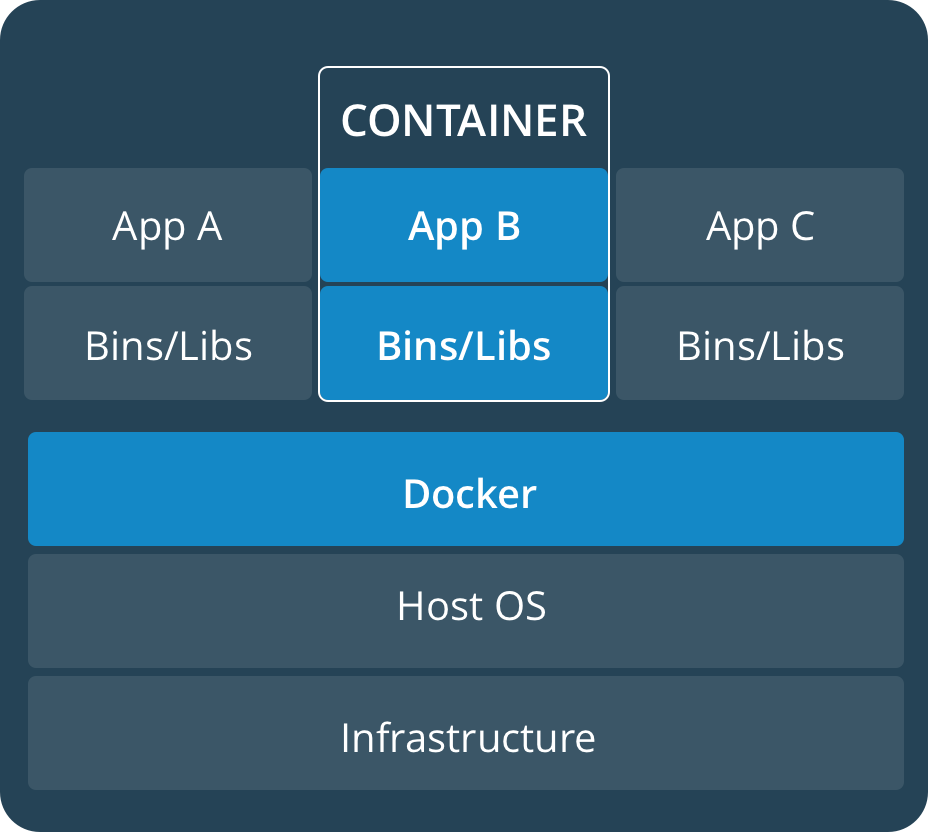
\includegraphics[width=0.4\textwidth]{container.png}
\caption{\label{fig:cont}Infraestructura de un contenedor.}
\end{figure}

A diferencia de las máquinas virtuales convencionales, las tecnologías de contenedores como Docker no incluyen un sistema operativo completo en su imagen, tan solo las librerías y configuraciones necesarias para su funcionamiento (se puede observar un esquema en la Figura~\ref{fig:cont}). Esto permite mejorar la eficiencia al no existir la sobrecarga que supone la interacción de las máquinas virtuales con el sistema operativo huésped (guest), ya que Docker es capaz de realizar una interacción directa con el Kernel Linux de la máquina anfitrión (host).

Algunas características destacadas sobre Docker en la conferencia son las siguientes: es portable, ligero, automatizable, autocontenido, aislado(ofrece entorno de desarrollo que se comporta a modo de \textit{sandbox}), agiliza el despliegue y el mantenimiento.

Con muchos contenedores pueden aparecer problemas de coordinación, para solucionarlos se utilizan balanceadores de carga o administradores (también conocidos como orquestadores). Algunos de los más conocidos son:
\begin{itemize}
\item Kubernetes (Google)
\item Amazon Web Services ECS
\item Docker Swarm
\end{itemize}

\subsection{Manual técnico de Docker}



\section{DevOps}\label{sec:devops}
%\todo[inline, color=green!40]{This is an inline comment.}

Otro de los conceptos introducidos en la conferencia es el de DevOps (el término proviene del acrónimo inglés formado por \textit{Development y Operations}), es un concepto que ha atraído un interés creciente en el ámbito de la gestión de proyectos y la ingeniería del Software durante la última década. Recibe una gran influencia de las metodologías ágiles de desarrollo y propone una mejora de la comunicación entre los equipos de desarrollo y operaciones. A lo largo de la historia, se ha producido un conflicto entre ambos equipos que surge de forma natural de sus roles, en el área de desarrollo se intenta introducir nueva funcionalidad mientras que el equipo de operaciones crea estabilidad y se ocupa de resolver errores. 

Las técnicas de DevOps se basan en la creación de una cultura común entre ambos equipos, que se aproveche al máximo de la automatización de procesos, la obtención de métricas que permita guiar la toma de decisiones y la integración de ambos equipos de forma que participen en todo el ciclo de vida del proyecto(diseño, desarrollo, mantenimiento…).

Una de las herramientas más utilizadas para automatizar las actividades del ciclo de vida del Software es Jenkins. Esta herramienta permite definir tareas para automatizar el proceso de compilación, \textit{testing}, despliegue y recopilación de métricas. Otras herramientas que pueden de resultar de utilidad son SonarQube(Análisis de calidad del código) y NexusOSS(Gestor de dependencias y artefactos).


\section{Conclusiones}\label{sec:conclu}

Me siento obligado a hacer una mención especial a los conferenciantes, ya que hicieron una exposición detallada tanto de la base teórica, como de la componente práctica del diseño de aplicaciones basadas en microservicios usando Docker, AWS y otros componentes de arquitecturas SOA de la suite de servicios de código abierto Netflix OSS. Realizaron una exposición muy interesante de los conceptos detrás de las arquitecturas basadas en microservicios y de diferentes técnicas que emplean las grandes empresas para automatizar el proceso de desarrollo. Aunque fue una charla de 3 horas, no se hizo nada larga y la gente estuvo atenta y participativa en todo momento. Me gustaría recomendar que en los próximos cursos del Máster en Ingeniería Informática se repita esta conferencia pero en el horario de clase, ya que me ha parecido de las más interesantes y enriquecedoras de este año a pesar de haber sido una conferencia optativa de la semana de la informática.

Según mi juicio, considero que uno de los principales motivos del éxito de los microservicios es que presenta una gran sinergia con el paradigma del Cloud Computing, y permite hacer un diseño modular de las aplicaciones que facilita de forma natural la división de trabajo en un reparto con objetivos claros y sencillos, sobre los que se puede hacer \textit{testing} de forma sencilla y corregir errores sin afectar a otros componentes del sistema.

Creo que la tecnología de virtualización basada en contenedores Docker ha sido una de las mejores herramientas de código abierto que han surgido en los últimos tiempos, considero crítica su capacidad para interactuar directamente con el kernel Linux (mejorando en gran medida el rendimiento de servidores que alojan aplicaciones de múltiples clientes). Además, creo que el diseño de aplicaciones basadas en microservicios con Docker facilita la automatización de gran parte del ciclo de vida Software, y está íntimamente relacionado con las técnicas de integración continua y DevOps. Las ventajas que me parecen más relevantes son: 

\begin{itemize}
\item La flexibilidad derivada de satisfacer todas las dependencias de una aplicación y poder desplegarla sin preocupación alguna en cualquier servidor me parece tremendamente útil
\item Facilita el desarrollo en un entorno local de pruebas totalmente aislado.
\item Permite el la realización de pruebas y tests de unidad de funcionalidades bien definidas e independientes. Esto facilita en gran medida el reparto de trabajo entre diferentes equipos de desarrollo que pueden progresar en paralelo.
\item La integración de código de forma automática con servicios de control de versiones con servicios como Jenkins y despliegue en un servidor Cloud o privado mediante contenedores que tienen todas las dependencias necesarias satisfechas para que se ejecute la aplicación.
\end{itemize}



En resumen, creo que ha sido una de las mejores conferencias a las que he acudido este año, esto me ha motivado enormemente para buscar información y completar la base de conocimiento que se transmitió en la misma. A mi parecer, las tecnologías relacionadas con el Cloud Computing tienen una enorme proyección de futuro y es el deber de cualquier ingeniero que se precie conocer las bases del diseño de aplicaciones que proveen servicios a millones de personas en Internet, y que no van a parar de crecer en el futuro inmediato. 

\begin{thebibliography}{1}
%\bibitem{key} description. \href{https://...}{Enlace}
\bibitem{cloudpatts}\textbf{Cloud Computing Patterns, Springer (2014)}. \textit{Fundamentals to Design, Build, and Manage Cloud Applications}. Authors: Christoph Fehling, Frank Leymann, Ralph Retter, Walter Schupeck and Peter Arbitter.
\bibitem{cloudfunds}\textbf{NIST definition of cloud computing (2011).} \textit{Mell P., Grance T.}
\bibitem{cloudview}\textbf{A view of cloud computing. Communications of the ACM (2010)}\textit{vol. 53, no 4, p. 50-58. ARMBRUST}, Michael, et al.
\bibitem{microbook}\textbf{Building Microservices (2015, 1st edition). O'Reilly Media, Inc.} \textit{Designing fine-grained systems}. Author: Sam Newman.
\bibitem{synapse}\textbf{Synapse: a microservices architecture for heterogeneous-database web applications (2015).}\textit{Viennot, Nicolas, et al. Proceedings of the Tenth European Conference on Computer Systems. ACM.}\href{https://github.com/nviennot/synapse}{ Proyecto en Github}. \href{http://viennot.com/synapse.pdf}{Paper}.
\bibitem{reliab}\href{https://blogs.microsoft.com/microsoftsecure/2012/09/12/fundamentals-of-cloud-service-reliability/}{Fundaments of Cloud Service Reliability}, Microsoft Secure Blog.
\bibitem{zdwt}\href{http://cloudpatterns.org/design_patterns/zero_downtime}{Zero Downtime}, cloudpatterns.org.
\bibitem{wscom}\href{http://www.service-architecture.com/articles/web-services/web_services_explained.html}{Web Services Explained} (Communication). service-architecture.com.
\bibitem{ibmsoa}\href{https://www-01.ibm.com/software/solutions/soa/}{Service Oriented Architecture}: simply good design. ibm.com.
\bibitem{sless}\href{http://www.cloudcomputingpatterns.org/stateless_component/}{Stateless Component, cloudcomputingpatterns.org}
\bibitem{restapi}\href{https://bbvaopen4u.com/es/actualidad/api-rest-que-es-y-cuales-son-sus-ventajas-en-el-desarrollo-de-proyectos}{API REST: ventajas.}  bbvaopen4u.com.
\bibitem{mservices}\href{https://martinfowler.com/articles/microservices.html}{Artículo sobre Microservicios y automatización}. Martin Fowler.
\end{thebibliography}

\end{document}